\subsection{Alpha Models}

A schematic of a live 'production' trading strategy is shown below, but does not include everything else necessary to create the strategy (i.e., research tools).
\begin{figure}[H]
\centering
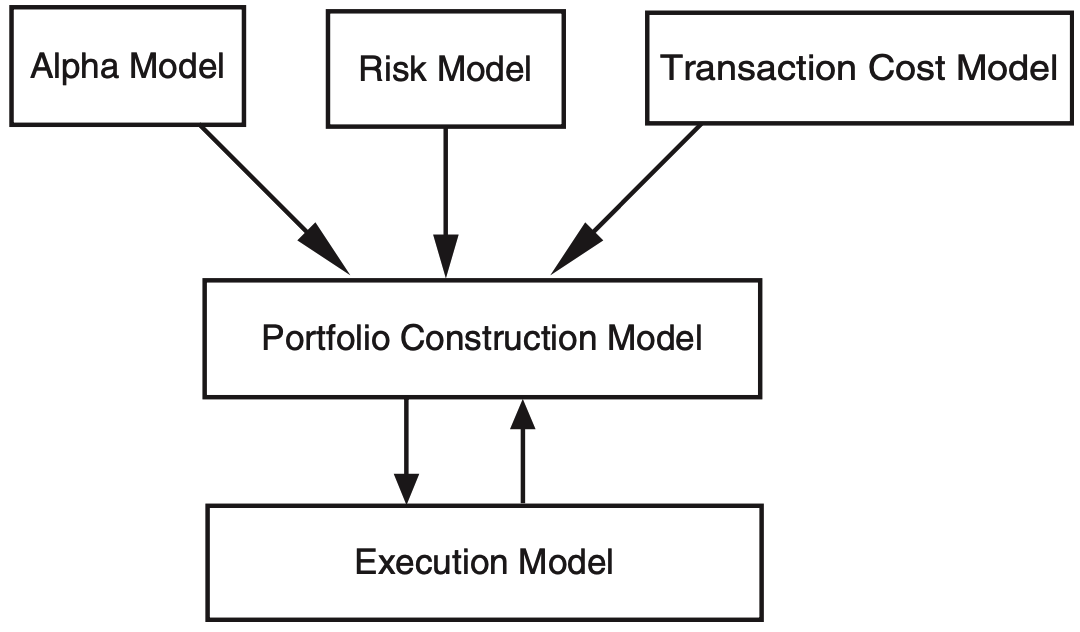
\includegraphics[scale=0.4]{fundamentals/strategystructure}
\caption{Live 'production' trading strategy}
\end{figure}
The trading system has three modules:
\begin{enumerate}[label=\roman*.]
\setlength{\itemsep}{0pt}
\item Alpha model: predicts the future of the instruments considered for trading, i.e. directional alpha
\item Risk model: limits amount of exposure to factors that are unlikely to generate returns but could drive losses, i.e. directional exposure limit on an asset class
\item Transaction cost model: determine if the cost of the trades needed to migrate from current portfolio to new portfolio is desirable to the portfolio construction model.
\end{enumerate}
These models feed into a portfolio construction model that balances the tradeoffs of profit and risk to determine the best portfolio to hold. The model finds the differences in trades that need to be executed.\\
The execution model then takes the required trades, and using inputs such as urgency in which the trades need to be executed and dynamics of liquidity in the markets, executes the trades in an efficient and low cost manner.

\subsubsection{Types of Models}

Theory-driven models tests theories of why markets behave in a manner, and see if they can be used to predict the future. Strategies utilising price-related data are trend and mean reversion; strategies utilising fundamental data are value/yield, growth and quality. Usually more than one model is used in combination.

\begin{definition}
\hlt{(Trend Following)} Markets move in given direction long enough that the trend can be identified. As more data support the bull/bear thesis in an uncertain market, more market participants will adopt the same thesis and hence move the asset price to a new equilibrium.
\end{definition}
An example of a trend is a moving average crossover indicator. This strategy has less than one point of return for every point of downside risk taken, as market behaviour are unstable and episodic.

\begin{definition}
\hlt{(Mean Reversion)} Markets move in opposite direction to the prevailing trend. Short-term imbalances between buyers and sellers due to liquidity forces prices to move abruptly in one direction, which increases probability of trend reversion as liquidity issue is resolved.
\end{definition}
An example of mean reversion strategy is statistical arbitrage, which bets on convergence of prices of similar stocks whose prices have diverged.\\

Trend and mean reversion strategies are not at odds. Longer-term trends can occur despite smaller oscillations around these trends occurring in the shorter term, hence both strategies may be use din conjunction.\\

\begin{definition}
\hlt{(Value/Yield)} Value strategies are usually ratios of some fundamental factor against the price of the instrument, inverted to keep the ratio consistent. The higher the yield, the cheaper the instrument.
\end{definition}
Market tend to overestimate risk in risky instruments and underestimate the risk in less risky instruments. When the strategy is executed on a relative basis, i.e., buying the undervalued security and selling the overvalued one against it, this is a \hlt{carry trade}. The difference between yield received and yield paid is the \hlt{carry}.\\

\hlt{Quant Long Short (QLS)} ranks stocks by attractiveness based on various factors such as value, then buy the higher-ranked stocks while shorting the lower-ranked stocks.

\begin{definition}
\hlt{(Growth)} Make predictions based on asset's expected or historically observed level of economic growth. Forward-looking growth expectations are typically used as a metric.
\end{definition}
Growth is trending, and strongest growers are becoming more dominant relative to competitors. Macro growth factors may be used on foreign exchange, while micro growth factors may be used on companies.

\begin{definition}
\hlt{(Quality)} All else being equal, it is better to long high quality and short low quality. Capital safety is important. Factors include earnings quality, equity-to-debt ratios etc.
\end{definition}

Data-driven models are more difficult to understand, with more complicated mathematics. Relies on data mining, more technically challenging and far less widely practiced. Typically more used in high-frequency space, as they can discern how market behaves without caring about the economic theory or rational.

\subsubsection{Strategy Implementation}

An implementation approach requires a forecast target, time horizon, bet structure, investment universe, model specification, and run frequency.\\

\hlt{(Forecast Target)} Models may forecast direction, magnitude, duration of move, and may include probability into the forecast. Signal strength is of importance, defined by a larger expected return and/or higher likelihood of return. A higher level of signal strength results in a bigger bet taken on the position.\\

\hlt{(Time Horizon)} Models may have forecast horizons ranging from microseconds to years. There are more variability between short-term and long-term strategies, as short-term strategies are making very large number of trades compared to long-term strategies.\\

\hlt{(Bet Structure)} Models can be made to forecast an instrument relative in itself or to others. For relative forecasts, smaller clusters (pairs) or larger clusters (sectors) may be used. For pairs, few assets can be compared precisely and directly. Large cluster grouping may eliminate impact of general movement of the sector and hence focus on the relative movement of stocks within the sector, allowing for clearer distinction between group behaviour and idiosyncratic behaviour. Clusters may be created either via statistical methods or using heuristics (i.e., fundamentally defined industry groups).\\
Statistical methods may be fooled by data, leading to bad grouping. Heuristic grouping may be imprecise for conglomerates, and may be too rigid. Relative alpha strategies tend to exhibit smoother returns during normal times than intrinsic alpha strategies, but may face incorrect groupings during stressful periods. This may be mitigated by utilising several grouping techniques in concert.\\

\hlt{(Investment Universe)} Choices made on geography, asset class, instrument class, and exclusions. Generally, liquidity is preferred so estimations of transaction costs are reliable. Large quantities of high quality data is required, which is found in highly liquid and developed markets. Instruments with consistent behaviour is preferred, hence biotech stocks are excluded due to sudden, violent price changes. Hence, the most common asset classes and instruments modelled are common stocks, futures (on bonds and equity indices) and forex.\\

\hlt{(Model Specification)} Focuses on definition of the strategy mathematically, and may be the source of alpha. Specification details in terms of machine learning or data mining techniques are also defined, to assist in fitting models to the data and setting parameter values. Refitting frequency is also defined to refresh the model and make it adapt to current market conditions; may lead to greater risk of overfitting.\\

\hlt{(Run Frequency)} Run frequency of model is defined, from monthly to real time frequency. Increasing frequency of runs lead to greater number of transactions and hence higher transaction costs, and risk of moving portfolio based on noisy data. Less frequency of runs lead to smaller number of larger-sized trades, hence may move the market with block trades; may also miss opportunities to trade at more favourable prices.

\subsubsection{Blending Models}

The three most common approaches are linear models, nonlinear models, and machine learning models. If models are not combined, then several portfolios are constructed based on output from each model, then combined using portfolio construction techniques. The best method depends on the model.

Linear models require independence of factors, and each factor to be additive. To determine the weight of each alpha factor, multiple regression techniques may be used.

Nonlinear models are used when factors are not independent, or the relationship changes over time. Conditional models base the weight of one factor on the reading of another factor. Rotational models assign weights of factors that fluctuate over time based on updated calculations of the various signal's weights, giving higher weights to factors with better performance recently.

Machine learning models applied to mixing alpha factors are more successful than the approach being used to forecast markets. For rotational models, many approaches to mixing alpha factors periodically update optimal weights based on the changing and growing dataset.


